\documentclass{article}
\usepackage{tikz}

\begin{document}

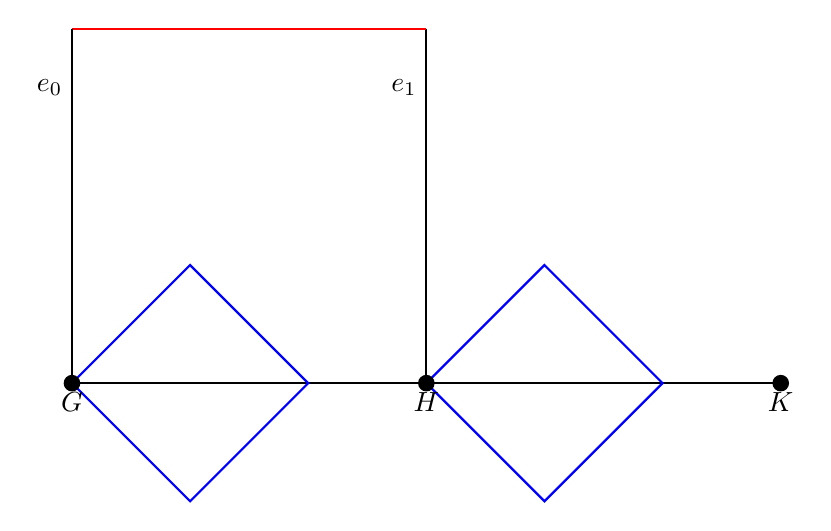
\begin{tikzpicture}[scale=1.5]
    % Define coordinates
    \coordinate (G) at (0,0);
    \coordinate (H) at (3,0);
    \coordinate (K) at (6,0);
    
    % Draw horizontal line
    \draw[thick] (G) -- (H) -- (K);
    
    % Draw vertical lines
    \draw[thick] (G) -- ++(0,3) coordinate (G1);
    \draw[thick] (H) -- ++(0,3) coordinate (H1);
    
    % Draw diagonal lines
    \draw[red, thick] (G1) -- (H1);
    
    % Draw diamond shapes
    \draw[blue, thick] (G) -- ++(1,1) -- ++(1,-1) -- ++(-1,-1) -- cycle;
    \draw[blue, thick] (H) -- ++(1,1) -- ++(1,-1) -- ++(-1,-1) -- cycle;
    
    % Label vertices
    \fill (G) circle (2pt) node[below] {$G$};
    \fill (H) circle (2pt) node[below] {$H$};
    \fill (K) circle (2pt) node[below] {$K$};
    
    % Label edges
    \draw (G1) -- ++(0,-1) node[midway, left] {$e_0$};
    \draw (H1) -- ++(0,-1) node[midway, left] {$e_1$};
\end{tikzpicture}

\end{document}